\chapter{Modelli dei Componenti e Quadripoli}
\label{ch:modelli-quadripoli}
\addtocontents{toc}{\protect\setcounter{tocdepth}{1}}
\section{Relazioni Tensione-Corrente e Modelli}

\subsection*{Componenti lineari}
Le relazioni tensione-corrente per i componenti base sono riassunte nella tabella seguente:
\begin{table}[H]
    \centering
    \renewcommand{\arraystretch}{1.5}
    \begin{tabular}{llc}
        \toprule
        \textbf{Componente} & \textbf{Relazione Tensione-Corrente} & \textbf{Simbolo Elettrico} \\
        \midrule
        \textbf{Resistenza} & $V(t) = R \, I(t)$ & \begin{circuitikz}[baseline=-0.5ex, scale=0.8, transform shape] \draw (0,0) to[R, v=$V$, i>=$I$] (2,0); \end{circuitikz} \\
        \textbf{Induttanza} & $V(t) = L \frac{dI(t)}{dt}$ & \begin{circuitikz}[baseline=-0.5ex, scale=0.8, transform shape] \draw (0,0) to[L, v=$V$, i>=$I$] (2,0); \end{circuitikz} \\
        \textbf{Condensatore} & $I(t) = C \frac{dV(t)}{dt}$ & \begin{circuitikz}[baseline=-0.5ex, scale=0.8, transform shape] \draw (0,0) to[C, v=$V$, i>=$I$] (2,0); \end{circuitikz} \\
        \textbf{Cortocircuito} & $V(t) = 0$ & \begin{circuitikz}[baseline=-0.5ex, scale=0.8, transform shape] \draw (0,0) to[short, i>=$I$] (2,0); \end{circuitikz} \\
        \textbf{Circuito aperto} & $I(t) = 0$ & \begin{circuitikz}[baseline=-0.5ex, scale=0.8, transform shape] \draw (0,0) to[open, v=$V$, o-o] (2,0); \end{circuitikz} \\
        \bottomrule
    \end{tabular}
    \caption{Simbologia e relazioni caratteristiche per i componenti lineari ideali bipolari.}
\end{table}

\subsection*{Componenti non lineari}

\textbf{Diodi:} Un diodo presenta un comportamento asimmetrico. In \textbf{Polarizzazione Diretta (PD)}, conduce corrente quando la tensione applicata supera la tensione di soglia ($V_{AK} \ge V_\gamma$). Se la tensione è inferiore alla soglia ($V_{AK} < V_\gamma$) la corrente è trascurabile; in particolare in \textbf{Polarizzazione Inversa (PI)}, cioè per $V_{AK} < 0$, scorre solo la piccolissima corrente inversa $-I_0$.

\begin{figure}[H]
    \centering
    \begin{circuitikz}[american, scale=1.2, transform shape]
        \draw (0,0) node[anchor=east]{Anodo ($A$)} to[D, v=$V_{AK}$, i>=$I(t)$, o-o] (3,0) node[anchor=west]{Catodo ($K$)};
    \end{circuitikz}
    \caption{Simbolo elettrico del diodo a giunzione PN. La freccia del simbolo indica il verso in cui è consentito il passaggio della corrente (polarizzazione diretta).}
\end{figure}

\subsection*{Diodo e Giunzioni}
\textbf{Modello di Shockley:} L'equazione esatta che descrive la caratteristica tensione-corrente di un diodo è l'equazione di Shockley:
$$ I(t) = I_0 \left[ \exp\left(\frac{V_{AK}}{\eta V_T}\right) - 1 \right] $$
dove $I_0$ è la corrente di saturazione inversa, $V_{AK}$ è la differenza di potenziale applicata ai capi del diodo (Anodo - Catodo), $V_T \simeq 26\,\text{mV}$ (a temperatura ambiente $T \simeq 300\,\text{K}$) è la tensione termica, e $\eta$ è il fattore di idealità ($\eta \simeq 2$ per il silicio, $\eta \simeq 1$ per il germanio).


\textbf{Retta di carico}
In un circuito base con un generatore di tensione $V_S$, una resistenza $R$ e un diodo in serie, il punto di lavoro (o punto di riposo) $(V_q, I_q)$ si ottiene mettendo a sistema l'equazione della retta di carico imposta dal circuito esterno e l'equazione caratteristica del diodo:
$$ \begin{cases}
V_{AK} = V_S - R I \\
I = I_0 \left[ \exp\left(\frac{V_{AK}}{\eta V_T}\right) - 1 \right]
\end{cases} $$
L'intersezione di queste due curve definisce il punto di lavoro (Quiescent point) $Q=(V_q, I_q)$.

\begin{figure}[H]
    \centering
    \begin{minipage}{0.4\textwidth}
        \centering
        \begin{circuitikz}[american, scale=1, transform shape]
            \draw (0,0) to[V, l=$V_S$] (0,3)
                  to[R, l=$R$] (3,3)
                  to[D, l=$D$, v=$V_{AK}$, i>=$I$] (3,0)
                  to[short] (0,0);
        \end{circuitikz}
    \end{minipage}%
    \begin{minipage}{0.55\textwidth}
        \centering
        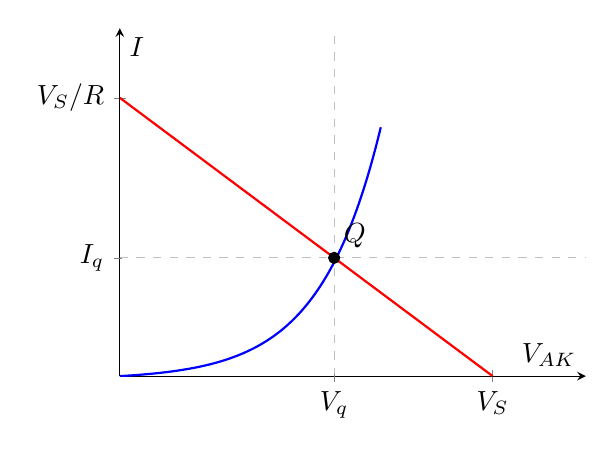
\begin{tikzpicture}
            \begin{axis}[
                axis lines = middle,
                xlabel = {$V_{AK}$},
                ylabel = {$I$},
                xmin=0, xmax=5,
                ymin=0, ymax=5,
                xtick={4}, xticklabels={$V_S$},
                ytick={4}, yticklabels={$V_S/R$},
                extra x ticks={2.3}, extra x tick labels={$V_q$},
                extra y ticks={1.7}, extra y tick labels={$I_q$},
                extra tick style={grid=major, dashed},
                width=7.5cm, height=6cm
            ]
            % Equazione di Shockley approssimata per disegno
            \addplot [domain=0:2.8, samples=100, color=blue, thick] {0.05 * exp(1.53*x) - 0.05};
            % Retta di carico
            \addplot [domain=0:4, color=red, thick] {-x + 4};
            
            % Punto di lavoro
            \addplot[mark=*] coordinates {(2.3,1.7)} node[above right] {$Q$};
            \end{axis}
        \end{tikzpicture}
    \end{minipage}
    \caption{Risoluzione grafica di un circuito non lineare elementare. Il punto di riposo (Quiescent point) $Q$ è individuato dall'intersezione tra l'equazione caratteristica del diodo (curva esponenziale blu) e l'equazione della retta di carico (retta rossa determinata da $V_S$ e $R$).}
\end{figure}

\textbf{Resistenza dinamica (Modello per piccoli segnali)}\\
Quando si studiano i piccoli segnali, dobbiamo \textbf{passivare i generatori DC} lasciando accesi solo i generatori AC.
Per piccole oscillazioni intorno al punto di lavoro, il diodo può essere \textit{linearizzato}. La corrente totale diventa la sovrapposizione della corrente di riposo e della piccola variazione dovuta al segnale (escursioni di corrente e tensione):
$$ I \simeq I_q + \left. \frac{dI}{dV_{AK}} \right|_q (V_{AK} - V_q) \quad \Rightarrow \quad I = I_q + i = I_q + \frac{v_{ak}}{r_d} $$
La grandezza $r_d$ è la \textbf{resistenza dinamica} del diodo, calcolata come l'inverso della derivata della caratteristica nel punto di lavoro:
$$ r_d = \left( \left. \frac{dI}{dV_{AK}} \right|_q \right)^{-1} = \left( \frac{I_0}{\eta V_T} \exp\left(\frac{V_q}{\eta V_T}\right) \right)^{-1} \simeq \frac{\eta V_T}{I_q} $$
Come si nota, la resistenza dinamica $r_d$ è inversamente proporzionale alla corrente di lavoro $I_q$: più corrente scorre nel diodo, più la sua resistenza dinamica è piccola.

\begin{figure}[H]
    \centering
    \begin{tikzpicture}
        \begin{axis}[
            axis lines = middle,
            xlabel = {$V_{AK}$},
            ylabel = {$I$},
            xmin=0, xmax=3,
            ymin=0, ymax=7,
            xtick={2}, xticklabels={$V_q$},
            ytick={4.017}, yticklabels={$I_q$},
            width=8cm, height=6.5cm,
            clip=false
        ]
        % Curva del diodo
        \addplot [domain=0:2.35, samples=100, color=blue, thick] {0.2*exp(1.5*x)};
        % Tangente
        \addplot [domain=1.5:2.5, color=green!60!black, thick, dashed] {6.025*x - 8.03} node[right] {pendenza $= \frac{1}{r_d}$};
        
        % Punto di lavoro
        \addplot[mark=*] coordinates {(2, 4.017)} node[left=3pt] {$Q$};
        
        % Annotazione per l'escursione di segnale
        \draw[<->, red, thick] (axis cs: 2, 4.017) -- (axis cs: 2.3, 4.017) node[midway, below] {$v_{ak}$};
        \draw[<->, red, thick] (axis cs: 2.3, 4.017) -- (axis cs: 2.3, 5.82) node[midway, right] {$i$};
        \end{axis}
    \end{tikzpicture}
    \caption{Linearizzazione per piccoli segnali (resistenza dinamica). Nell'intorno del punto di lavoro $Q$, piccole variazioni di tensione e corrente ($v_{ak}$ e $i$) consentono di approssimare la curva esponenziale tramite la sua retta tangente, il cui coefficiente angolare è l'inverso della resistenza dinamica $r_d$.}
\end{figure}

\section{Quadripoli o Doppi Bipoli}
Un quadripolo è un componente o un circuito visto dall'esterno tramite quattro morsetti, raggruppati in due porte: due morsetti formano la porta d'ingresso e due la porta d'uscita. In ogni porta la corrente che entra da un morsetto esce dall'altro; per convenzione le correnti $I_1$ e $I_2$ sono considerate \emph{entranti} nel quadripolo.

Analogamente a quanto visto per il diodo, possiamo descrivere le equazioni del quadripolo sfruttando un'espansione di Taylor (linearizzazione) nell'intorno di un punto di lavoro $Q$. A seconda di quali variabili (correnti o tensioni) scegliamo come indipendenti, otteniamo diversi modelli matematici e matrici caratteristiche.

\subsection{Modelli dei Quadripoli}

Si ricorda la dualità tra resistenza e conduttanza (e tra impedenza e ammettenza):
$$ R \,(\text{resistenza}) \xleftrightarrow{\hspace*{0.3cm} (\cdot)^{-1} \hspace*{0.3cm}} G \,(\text{conduttanza}) \quad ; \quad Z \,(\text{impedenza}) \xleftrightarrow{\hspace*{0.3cm} (\cdot)^{-1} \hspace*{0.3cm}} Y \,(\text{ammettenza}) $$

\subsubsection*{Modello a parametri Y (Ammettenze)}
I quadripoli possono essere caratterizzati fissando le tensioni $V_1$ e $V_2$ alle due porte. Le correnti sono considerate variabili dipendenti: $I_i = f(V_1, V_2)$.
    
\begin{figure}[H]
    \centering
    \begin{circuitikz}[american, scale=1.2, transform shape]
        % Scatola centrale
        \draw (2,1) rectangle (4,3);
        \node at (3,2) {\Large $Y$};
        % Porta di ingresso
        \draw (0,2.5) to[short, o-, i=$I_1$] (2,2.5);
        \draw (0,1.5) to[short, o-] (2,1.5);
        \draw[<->] (0,2.4) -- (0,1.6) node[midway, left] {$V_1$};
        % Porta di uscita
        \draw (6,2.5) to[short, o-, i=$I_2$] (4,2.5);
        \draw (6,1.5) to[short, o-] (4,1.5);
        \draw[<->] (6,2.4) -- (6,1.6) node[midway, right] {$V_2$};
    \end{circuitikz}
    \caption{Schema a blocchi descritto mediante i parametri di ammettenza $Y$. Variabili indipendenti: $V_1, V_2$.}
\end{figure}
    
Linearizzando per piccoli segnali otteniamo:
$$ I_i \simeq I_{qi} + \sum_j \left. \frac{\partial I_i}{\partial V_j} \right|_q (V_j - V_{qj}) \quad \Rightarrow \quad i_i = \left. \frac{\partial I_i}{\partial V_1} \right|_q v_1 + \left. \frac{\partial I_i}{\partial V_2} \right|_q v_2 \equiv \sum_j Y_{ij} v_j $$
I parametri della matrice delle ammettenze $Y$ sono definiti come le derivate parziali calcolate nel punto di lavoro:
$$ Y_{ij} = \left. \frac{\partial I_i}{\partial V_j} \right|_q $$

\subsubsection*{Modello a parametri Z (Impedenze)}
Questo modello è caratterizzato fissando le correnti $I_1$ e $I_2$ alle porte d'ingresso e d'uscita. Le tensioni sono in questo caso le variabili dipendenti: $V_i = f(I_1, I_2)$.
    
\begin{figure}[H]
    \centering
    \begin{circuitikz}[american, scale=1.2, transform shape]
        % Scatola centrale
        \draw (2,1) rectangle (4,3);
        \node at (3,2) {\Large $Z$};
        % Porta di ingresso
        \draw (0,2.5) to[short, o-, i=$I_1$] (2,2.5);
        \draw (0,1.5) to[short, o-] (2,1.5);
        \draw[<->] (0,2.4) -- (0,1.6) node[midway, left] {$V_1$};
        % Porta di uscita
        \draw (6,2.5) to[short, o-, i=$I_2$] (4,2.5);
        \draw (6,1.5) to[short, o-] (4,1.5);
        \draw[<->] (6,2.4) -- (6,1.6) node[midway, right] {$V_2$};
    \end{circuitikz}
    \caption{Modello a parametri impedenze $Z$. Variabili indipendenti: $I_1, I_2$.}
\end{figure}
    
Linearizzando per piccoli segnali:
$$ V_i \simeq V_{qi} + \sum_j \left. \frac{\partial V_i}{\partial I_j} \right|_q (I_j - I_{qj}) \quad \Rightarrow \quad v_i = \left. \frac{\partial V_i}{\partial I_1} \right|_q i_1 + \left. \frac{\partial V_i}{\partial I_2} \right|_q i_2 \equiv \sum_j Z_{ij} i_j $$
I parametri della matrice delle impedenze $Z$ sono pertanto:
$$ Z_{ij} = \left. \frac{\partial V_i}{\partial I_j} \right|_q $$
\begin{note}Analogamente alle equivalenze di Thevenin-Norton, esistono idealmente casi di singolarità in cui le suddette matrici non risultano invertibili.\end{note}

\subsubsection*{Modello a parametri H (Ibrido)}
Il modello ibrido si ottiene fissando come variabili indipendenti miste $I_1$ all'ingresso e $V_2$ in uscita.
    
\begin{figure}[H]
    \centering
    \begin{circuitikz}[american, scale=1.2, transform shape]
        % Scatola centrale
        \draw (2,1) rectangle (4,3);
        \node at (3,2) {\Large $H$};
        % Porta di ingresso
        \draw (0,2.5) to[short, o-, i=$I_1$] (2,2.5);
        \draw (0,1.5) to[short, o-] (2,1.5);
        \draw[<->] (0,2.4) -- (0,1.6) node[midway, left] {$V_1$};
        % Porta di uscita
        \draw (6,2.5) to[short, o-, i=$I_2$] (4,2.5);
        \draw (6,1.5) to[short, o-] (4,1.5);
        \draw[<->] (6,2.4) -- (6,1.6) node[midway, right] {$V_2$};
    \end{circuitikz}
    \caption{Modello a parametri Ibridi $H$. Variabili indipendenti: $I_1, V_2$.}
\end{figure}
    
Partendo dalle relazioni base in cui $V_1 = f(I_1, V_2)$ e $I_2 = f(I_1, V_2)$, per piccoli segnali si definiscono i parametri $h_{ij}$:
$$ v_1 = \left. \frac{\partial V_1}{\partial I_1} \right|_q i_1 + \left. \frac{\partial V_1}{\partial V_2} \right|_q v_2 $$
$$ i_2 = \left. \frac{\partial I_2}{\partial I_1} \right|_q i_1 + \left. \frac{\partial I_2}{\partial V_2} \right|_q v_2 $$
La matrice $H$ risultante è ibrida, e di conseguenza i suoi coefficienti possiedono dimensioni fisiche eterogenee (es. impedenze, ammettenze, guadagni puri).

\subsubsection*{Modello a parametri M (Ibrido Inverso)}
In modo analogo ma invertito, questo modello fissa come variabili indipendenti $V_1$ all'ingresso e $I_2$ in uscita.
    
\begin{figure}[H]
    \centering
    \begin{circuitikz}[american, scale=1.2, transform shape]
        % Scatola centrale
        \draw (2,1) rectangle (4,3);
        \node at (3,2) {\Large $M$};
        % Porta di ingresso
        \draw (0,2.5) to[short, o-, i=$I_1$] (2,2.5);
        \draw (0,1.5) to[short, o-] (2,1.5);
        \draw[<->] (0,2.4) -- (0,1.6) node[midway, left] {$V_1$};
        % Porta di uscita
        \draw (6,2.5) to[short, o-, i=$I_2$] (4,2.5);
        \draw (6,1.5) to[short, o-] (4,1.5);
        \draw[<->] (6,2.4) -- (6,1.6) node[midway, right] {$V_2$};
    \end{circuitikz}
    \caption{Modello a parametri Ibridi Inversi $M$. Variabili indipendenti: $V_1, I_2$.}
\end{figure}
    
Partendo dalle relazioni duali $I_1 = f(V_1, I_2)$ e $V_2 = f(V_1, I_2)$, andiamo a definire i parametri $m_{ij}$:
$$ i_1 = \left. \frac{\partial I_1}{\partial V_1} \right|_q v_1 + \left. \frac{\partial I_1}{\partial I_2} \right|_q i_2 $$
$$ v_2 = \left. \frac{\partial V_2}{\partial V_1} \right|_q v_1 + \left. \frac{\partial V_2}{\partial I_2} \right|_q i_2 $$
La matrice $M$ costituisce la matrice ibrida inversa, condividendo anch'essa l'eterogeneità dimensionale dei coefficienti.

\subsection{Caratterizzazione sperimentale dei parametri}
Come facciamo a misurare e caratterizzare i parametri di questi modelli mediante misure in laboratorio?
Si procede annullando di volta in volta una delle variabili indipendenti (creando cortocircuiti o circuiti aperti per i piccoli segnali).

\paragraph{Esempio per i parametri $H$}
Per ricavare i quattro parametri della matrice ibrida $H$, occorre misurare il rapporto tra tensioni e correnti imponendo condizioni specifiche (zero) sulle variabili indipendenti non coinvolte:
Per misurare $h_{11} = \left. \frac{v_1}{i_1} \right|_{v_2=0}$ e $h_{21} = \left. \frac{i_2}{i_1} \right|_{v_2=0}$, è necessario annullare la tensione in uscita $v_2$, operazione che si ottiene ponendo la porta 2 in \textbf{cortocircuito} per i piccoli segnali. 
In modo complementare, per ottenere $h_{12} = \left. \frac{v_1}{v_2} \right|_{i_1=0}$ e $h_{22} = \left. \frac{i_2}{v_2} \right|_{i_1=0}$, bisogna annullare la corrente di ingresso $i_1$, lasciando la porta 1 a \textbf{circuito aperto}.

\paragraph{Estensione agli altri modelli}
La logica procedurale è identica per le altre rappresentazioni matematiche. Nel caso della matrice delle ammettenze $Y$, ogni parametro $Y_{ij} = \left. \frac{i_i}{v_j} \right|_{v_{k \neq j} = 0}$ si misura spegnendo il generatore in alternata $v_k$, ponendo quindi la rispettiva porta in cortocircuito. Viceversa, per i parametri di impedenza $Z_{ij} = \left. \frac{v_i}{i_j} \right|_{i_{k \neq j} = 0}$, si annulla la corrente $i_k$ mantenendo la porta corrispondente a circuito aperto.

\subsection{Teorema di Sostituzione}
\label{sec:sostituzione}
Se in un circuito un bipolo è attraversato dalla corrente $I$ e ha ai capi la tensione $V$, lo si può sostituire con un generatore di corrente $I$ oppure con un generatore di tensione $V$ senza cambiare le altre grandezze del circuito: le equazioni di maglia e di nodo restano le stesse. In particolare la caduta $RI$ su una resistenza può essere schematizzata con un generatore di tensione dipendente dalla corrente (concetto base per i modelli dei transistor).
\begin{figure}[H]
    \centering
    \begin{circuitikz}[american, scale=1.0, transform shape]
        % Circuito 1: Resistenza
        \draw (0,1.5) rectangle (1.5,2.5);
        \draw (1.5,2) to[R, l=$R$, i=$I$, -o] (3.5,2);
        
        \node at (4,2) {$\iff$};
        
        % Circuito 2: Generatore di corrente (ideal)
        \draw (4.5,1.5) rectangle (6,2.5);
        \draw (6,2) to[I, l=$I$, -o] (8,2);
        
        \node at (8.5,2) {$\iff$};
        
        % Circuito 3: Generatore di tensione dipendente
        \draw (9,1.5) rectangle (10.5,2.5);
        \draw (10.5,2) to[cV, l=$R I$, -o] (12.5,2); % Generatore dipendente (rombo)
    \end{circuitikz}
    \caption{Equivalenze secondo il Teorema di Sostituzione. Notare l'uso del generatore dipendente (simbolo a rombo).}
\end{figure}

\subsection{Rappresentazione a Piccolo Segnale: Modello H}
Il modello a parametri ibridi $H$ si rappresenta circuitalmente nel modo seguente:
\begin{figure}[H]
    \centering
    \begin{circuitikz}[american, scale=1.2, transform shape]
        % Porta 1
        \draw (0,2) to[short, o-, i=$i_1$] (1,2) 
              to[R, l=$h_{11}$] (3,2) 
              to[cV, l_=$h_{12}v_2$] (3,0) 
              to[short, -o] (0,0);
        \draw[<->] (0,1.8) -- (0,0.2) node[midway, left] {$v_1$};
        
        % Porta 2
        \draw (8,2) to[short, o-, i=$i_2$] (7,2);
        \draw (7,2) to[short] (5,2) 
              to[cI, l=$h_{21}i_1$] (5,0) 
              to[short] (7,0)
              to[short, -o] (8,0);
        \draw (7,2) to[R, l=$\frac{1}{h_{22}}$] (7,0);
        \draw[<->] (8,1.8) -- (8,0.2) node[midway, right] {$v_2$};
    \end{circuitikz}
    \caption{Circuito equivalente a piccolo segnale per il modello a parametri ibridi $H$.}
\end{figure}
Come visto in precedenza, le equazioni sono:
$$ v_1 = \left. \frac{\partial V_1}{\partial I_1} \right|_q i_1 + \left. \frac{\partial V_1}{\partial V_2} \right|_q v_2 = h_{11} i_1 + h_{12} v_2 $$
$$ i_2 = \left. \frac{\partial I_2}{\partial I_1} \right|_q i_1 + \left. \frac{\partial I_2}{\partial V_2} \right|_q v_2 = h_{21} i_1 + h_{22} v_2 $$

\subsubsection{Esempio: Partitore di tensione come quadripolo}
\begin{figure}[H]
    \centering
    \begin{circuitikz}[american]
        % Scatola tratteggiata
        \draw[dashed, gray] (1.5,-0.5) rectangle (3.5,2.5);
        \draw (0,2) to[short, o-, i=$i_1$] (1.5,2) 
              to[generic, l=$Z_1$] (3,2)
              to[short, -o, i<=$i_2$] (5,2);
        \draw (3,2) to[generic, l=$Z_2$] (3,0);
        \draw (0,0) to[short, o-o] (5,0);
        
        \draw[<->] (0,1.8) -- (0,0.2) node[midway, left] {$v_1$};
        \draw[<->] (5,1.8) -- (5,0.2) node[midway, right] {$v_2$};
    \end{circuitikz}
    \caption{Partitore di tensione visto come quadripolo.}
\end{figure}
Calcoliamo i parametri $H$:
Per determinare $h_{11} = Z_1$, si considera il cortocircuito $v_2$, in modo che $i_1$ attraversi solamente $Z_1$ e poi si scarichi a massa nel corto.
Il parametro $h_{12} = 1$ viene ottenuto lasciando il circuito aperto alla porta 1: in questa condizione non vi è caduta di tensione su $Z_1$ e l'intera tensione ricade su $Z_2$, per cui $v_1 = v_2$.
Imponendo nuovamente il cortocircuito su $v_2$, deduciamo $h_{21} = -1$: l'intera corrente $i_1$ esce dalla porta 2 attraverso il corto (in $Z_2$ non scorre corrente), quindi $i_2 = -i_1$ (ricordando che $i_2$ è presa entrante).
Infine, calcoliamo $h_{22} = \frac{1}{Z_2}$ imponendo un circuito aperto alla porta 1, situazione in cui la corrente $i_2$ attraversa unicamente l'impedenza $Z_2$.

\subsection{Amplificatore di Tensione}
Un amplificatore reale pilotato da un generatore reale ($V_S, R_S$) e chiuso su un carico ($R_L$).
\begin{figure}[H]
    \centering
    \begin{circuitikz}[american, scale=1.2, transform shape]
        % Generatore
        \draw (0,2) to[V, l=$V_S$] (0,0);
        \draw (0,2) to[R, l=$R_S$, i=$i_1$] (2,2);
        \draw (0,0) to[short] (2,0);
        
        % Porta d'ingresso
        \draw (2,2) to[short, o-] (2.5,2);
        \draw (2,0) to[short, o-] (2.5,0);
        
        % Blocco Amplificatore
        \draw (2.5,0) rectangle (4.5,2);
        \node at (3.5,1) {Ampl.};
        
        % Porta d'uscita
        \draw (4.5,2) to[short, -o] (5,2);
        \draw (4.5,0) to[short, -o] (5,0);
        
        % Carico
        \draw (5,2) to[short, i=$i_2$] (7,2);
        \draw (5,0) to[short] (7,0);
        \draw (7,2) to[R, l_=$R_L$] (7,0);
        
        % Etichette tensioni
        \draw[<->] (2,1.8) -- (2,0.2) node[midway, left] {$v_1$};
        \draw[<->] (5,1.8) -- (5,0.2) node[midway, left] {$v_2$};
        \draw[<->] (7.5,1.8) -- (7.5,0.2) node[midway, right] {$V_{out}$};
    \end{circuitikz}
    \caption{Amplificatore di tensione inserito tra sorgente e carico.}
\end{figure}
Il guadagno in tensione è $A_V = \frac{V_{out}}{V_S}$.
Chiamando $|H| = h_{11}h_{22} - h_{12}h_{21}$ il determinante della matrice $H$:

\paragraph{Calcolo in condizioni ideali:} 
Se consideriamo $R_L = \infty$ e $R_S = 0$, e sapendo che $V_S = v_1$ e $V_{out} = v_2$, si ottiene $i_2 = 0$. Questo implica che $i_1 = - \frac{h_{22}}{h_{21}} v_2$, e di conseguenza $v_1 = \frac{h_{21}h_{12} - h_{11}h_{22}}{h_{21}} v_2$.
Il guadagno in tensione assume quindi la forma:
$$ A_V = \frac{v_2}{v_1} = \frac{h_{21}}{h_{21}h_{12} - h_{11}h_{22}} = - \frac{h_{21}}{|H|} $$
    
\paragraph{Calcolo in condizioni non ideali in uscita:} 
Considerando $R_L < \infty$ e mantenendo $R_S = 0$, possiamo sfruttare l'equivalente di Thevenin (\cref{sec:thevenin}). La tensione a circuito aperto è $V_T = v_2 (\text{aperto}) = - \frac{h_{21}}{|H|} v_1$. La resistenza d'uscita è $R_T = \frac{h_{11}}{|H|}$.
La tensione di uscita diventa:
$$ V_{out} = \frac{R_L}{R_L + R_T} V_T = - \frac{h_{21}}{|H|} v_1 \frac{R_L}{R_L + \frac{h_{11}}{|H|}} = - \frac{h_{21} v_1}{|H| + h_{11}/R_L} $$
Essendo $V_S = v_1$, il guadagno risulta:
$$ A_V = \frac{V_{out}}{V_S} = - \frac{h_{21}}{|H| + h_{11}/R_L} $$
    
\paragraph{Calcolo in condizioni non ideali in ingresso:} 
Infine, analizzando il caso duale con $R_L = \infty$ e $R_S > 0$, vale la relazione $v_1 = V_S - i_1 R_S$. Ponendo l'impedenza di ingresso $Z_{in} = \frac{v_1}{i_1}$, ricaviamo:
$$ V_S = \left( 1 + \frac{R_S}{Z_{in}} \right) v_1 \implies A_V = \frac{v_2}{V_S} = - \frac{h_{21}}{|H| + h_{22}R_S} $$

\subsection{Amplificatori a Cascata e Filtri}
Quando due stadi amplificatori sono collegati in cascata, il guadagno complessivo non è semplicemente il prodotto dei guadagni isolati: occorre tenere conto dell'interazione tra i due stadi attraverso il \textbf{fattore di partizione}, che dipende dall'adattamento d'impedenza tra i blocchi:
\begin{equation}
    A_\text{cas} = A_1 \cdot A_2 \cdot \underbrace{\frac{Z_{in}^{(2)}}{Z_{in}^{(2)} + Z_{out}^{(1)}}}_{\text{fattore di carico}}
\end{equation}
Qui $A_1$ e $A_2$ sono i guadagni a vuoto dei due stadi. Il fattore di carico tende a 1 solo nel caso ideale $Z_{out}^{(1)} \ll Z_{in}^{(2)}$. In tutti gli altri casi riduce il guadagno effettivo. Questo termine è fondamentale nell'analisi del filtro passa-banda.

\subsubsection{Filtro Passa-Basso (LP)}
La cella RC passa-basso lascia passare le frequenze $\omega \ll \omega_{LP} = 1/(RC)$ e attenua progressivamente quelle superiori. Il condensatore, con impedenza $Z_C = 1/(i\omega C)$ decrescente all'aumentare di $\omega$, devia la corrente verso massa per le alte frequenze.

\begin{figure}[H]
    \centering
    \begin{circuitikz}[american, scale=1.1, transform shape]
        \draw (0,2) to[short, o-] (0.5,2)
                    to[R, l=$R$] (3,2)
                    to[short, -o] (4,2);
        \draw (3,2) to[C, l=$C$, *-] (3,0) node[ground]{};
        \draw (0,0) node[ground]{} to[short, o-] (0,0);
        \draw[<->] (-0.5,1.8) -- (-0.5,0.05) node[midway,left]{$v_{in}$};
        \draw[<->] (4.5,1.8) -- (4.5,0.05) node[midway,right]{$v_{out}$};
    \end{circuitikz}
    \caption{Cella passa-basso passiva (RC). La funzione di trasferimento è $A_{LP} = 1/(1+i\omega/\omega_{LP})$, con $\omega_{LP}=1/(RC)$. Al di sopra di $\omega_{LP}$ il guadagno cala di $-20\,\mathrm{dB/decade}$.}
\end{figure}

Le impedenze equivalenti viste dalle porte del quadripolo sono:
\begin{align}
    Z_{in}^{LP} &= R + \frac{1}{i\omega C} = \frac{Z_C}{A_{LP}}, &
    Z_{out}^{LP} &= R \parallel \frac{1}{i\omega C} = A_{LP}\cdot R
\end{align}

\subsubsection{Filtro Passa-Alto (HP)}
La cella CR passa-alto blocca la componente continua e le basse frequenze $\omega \ll \omega_{HP} = 1/(RC)$. Alle alte frequenze il condensatore si comporta come un cortocircuito e $v_{out} \approx v_{in}$.

\begin{figure}[H]
    \centering
    \begin{circuitikz}[american, scale=1.1, transform shape]
        \draw (0,2) to[short, o-] (0.5,2)
                    to[C, l=$C$] (2.5,2)
                    to[short, -o] (4,2);
        \draw (2.5,2) to[R, l=$R$, *-] (2.5,0) node[ground]{};
        \draw (0,0) node[ground]{} to[short, o-] (0,0);
        \draw[<->] (-0.5,1.8) -- (-0.5,0.05) node[midway,left]{$v_{in}$};
        \draw[<->] (4.5,1.8) -- (4.5,0.05) node[midway,right]{$v_{out}$};
    \end{circuitikz}
    \caption{Cella passa-alto passiva (CR). La funzione di trasferimento è $A_{HP} = (i\omega/\omega_{HP})/(1+i\omega/\omega_{HP})$, con $\omega_{HP}=1/(RC)$. Al di sotto di $\omega_{HP}$ il modulo segue una retta di pendenza $+20\,\mathrm{dB/decade}$ (cioè cala di $20$\,dB per ogni decade verso le basse frequenze).}
\end{figure}

Le impedenze equivalenti sono:
\begin{align}
    Z_{in}^{HP} &= R + \frac{1}{i\omega C} = \frac{R}{A_{HP}}, &
    Z_{out}^{HP} &= R \parallel \frac{1}{i\omega C} = A_{HP}\cdot Z_C
\end{align}

\subsubsection{Filtro Passa-Banda (Cascata LP--HP)}
Il filtro passa-banda si ottiene collegando in cascata uno stadio passa-basso (Stadio~1) e uno stadio passa-alto (Stadio~2). Lo Stadio~1 taglia le frequenze troppo alte; lo Stadio~2 taglia le frequenze troppo basse. La frequenza di centro-banda è $\bar{\omega} = \sqrt{\omega_{LP}\,\omega_{HP}}$.

\begin{figure}[H]
    \centering
    \begin{circuitikz}[american, scale=1.05, transform shape]
        % --- Stadio 1: LP ---
        \draw[dashed, gray!60, rounded corners=4pt]
            (-0.3, -0.8) rectangle (2.6, 3.5);
        \node[gray!70, font=\small\itshape] at (1.15, 3.1) {Stadio 1 (LP)};
        
        \draw (0,2) to[short, o-] (0.5,2)
                    to[R, l=$R_1$] (2.2,2);
        \draw (2.2,2) to[C, l_=$C_1$, *-*] (2.2,0);
        \draw (0,0) to[short, o-*] (2.2,0);
        \draw (2.2,0) node[ground]{};
        
        % Collegamento tra i due stadi
        \draw (2.2,2) to[short] (3.0,2);
        \draw (2.2,0) to[short] (3.0,0);
        
        % --- Stadio 2: HP ---
        \draw[dashed, gray!60, rounded corners=4pt]
            (2.7, -0.8) rectangle (6.4, 3.5);
        \node[gray!70, font=\small\itshape] at (4.55, 3.1) {Stadio 2 (HP)};
        
        \draw (3.0,2) to[C, l=$C_2$] (4.6,2)
                      to[short, -o] (6.1,2);
        \draw (4.6,2) to[R, l_=$R_2$, *-*] (4.6,0);
        \draw (3.0,0) to[short] (4.6,0)
                      to[short, -o] (6.1,0);
        \draw (4.6,0) node[ground]{};
        
        % Etichette di tensione
        \draw[<->] (-0.6,1.8) -- (-0.6,0.2) node[midway,left]{$v_{in}$};
        \draw[<->] (6.6,1.8) -- (6.6,0.2) node[midway,right]{$v_{out}$};
    \end{circuitikz}
    \caption{Filtro passa-banda ottenuto dalla cascata LP--HP. Lo Stadio~1 (tratteggio sinistro) è un passa-basso RC; lo Stadio~2 (tratteggio destro) è un passa-alto CR. I due stadi interagiscono tramite il fattore di partizione $Z_{in}^{(2)}/(Z_{in}^{(2)}+Z_{out}^{(1)})$.}
\end{figure}

Le matrici ibride $H$ dei due stadi sono:
\[
    H_1 = \begin{pmatrix} R_1 & 1 \\ -1 & i\omega C_1 \end{pmatrix}, \qquad
    H_2 = \begin{pmatrix} (i\omega C_2)^{-1} & 1 \\ -1 & R_2^{-1} \end{pmatrix}
\]
I guadagni isolati dei due stadi risultano:
\[
    A_1(\omega) = \frac{1}{1 + i\omega/\omega_{LP}}, \qquad
    A_2(\omega) = \frac{i\omega/\omega_{HP}}{1 + i\omega/\omega_{HP}}
\]
Dalle relazioni matriciali ($Z_{in}Z_{out} = h_{11}/h_{22}$) si ricavano le impedenze:
\begin{align}
    Z_{out}^{(1)} &= A_1 R_1, & Z_{in}^{(1)} &= \frac{R_1}{1 - A_1} \\
    Z_{in}^{(2)}  &= \frac{R_2}{A_2}, & Z_{out}^{(2)} &= \left(\frac{1}{R_2} + i\omega C_2\right)^{-1}
\end{align}
Sostituendo nella formula del partitore per la cascata, il guadagno del passa-banda è:
\begin{align}
    A_{BP} &= A_1 A_2 \cdot \frac{Z_{in}^{(2)}}{Z_{in}^{(2)} + Z_{out}^{(1)}}
            = \frac{A_{LP}\,A_{HP}}{1 + \dfrac{R_1}{R_2}\,A_{LP}\,A_{HP}}
\end{align}

\subsubsection{Analisi della Funzione di Trasferimento del Passa-Banda}
Per $R_1 = R_2$ la funzione di trasferimento si semplifica:
\begin{align}
    T_{BP}(\omega)
    &= \frac{A_{LP}\,A_{HP}}{1 + A_{LP}\,A_{HP}} \nonumber\\[4pt]
    &= \frac{1}{2 + \dfrac{\omega_{HP}}{\omega_{LP}}
               + i\!\left(\dfrac{\omega}{\omega_{LP}} - \dfrac{\omega_{HP}}{\omega}\right)}
\end{align}
La parte reale del denominatore è costante, quindi il modulo $|T_{BP}|$ è massimo quando la parte immaginaria al denominatore si annulla:
\[
    \frac{\omega}{\omega_{LP}} - \frac{\omega_{HP}}{\omega} = 0
    \;\Longrightarrow\; \boxed{\omega = \bar{\omega} = \sqrt{\omega_{LP}\,\omega_{HP}}}
\]
In $\bar{\omega}$, la funzione è reale pura e vale $T_{BP}(\bar\omega) = \dfrac{1}{2 + \omega_{HP}/\omega_{LP}} \simeq \dfrac12$ (per $\omega_{HP} \ll \omega_{LP}$), quindi il segnale non subisce sfasamento. Alle frequenze di taglio $\omega'_{HP}$ e $\omega'_{LP}$ il guadagno scende a $1/\sqrt{2}$ del massimo ($-3\,\mathrm{dB}$) e lo sfasamento è di $\mp 45^\circ$.

\begin{figure}[H]
    \centering
    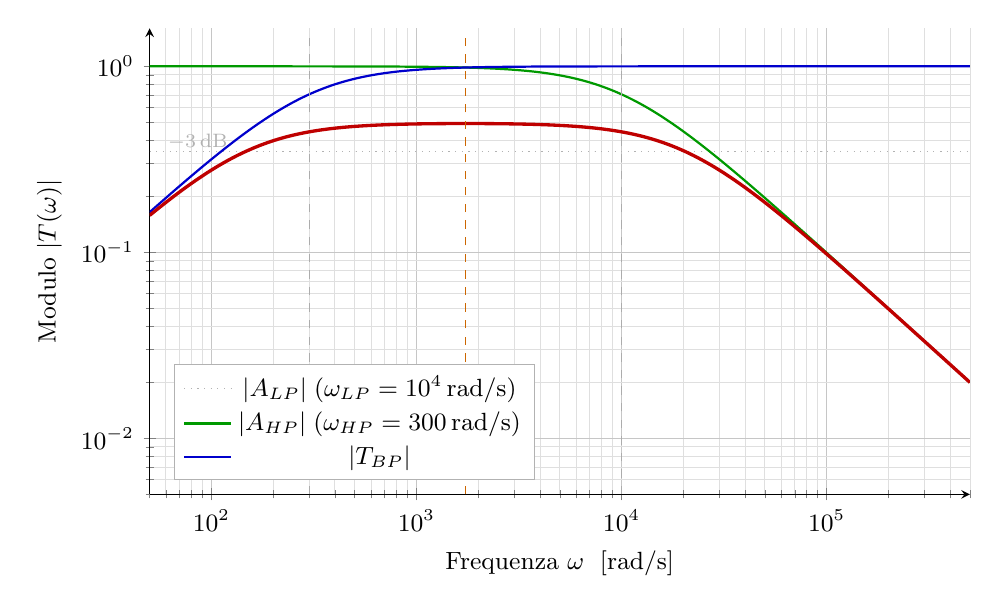
\begin{tikzpicture}
        \begin{axis}[
            xmode=log, ymode=log,
            domain=50:500000,
            samples=200,
            width=12cm, height=7.5cm,
            xlabel={Frequenza $\omega$ \;[rad/s]},
            ylabel={Modulo $|T(\omega)|$},
            xmin=50, xmax=500000,
            ymin=0.005, ymax=1.6,
            axis lines=left,
            grid=both,
            grid style={line width=0.3pt, draw=gray!25},
            major grid style={line width=0.5pt, draw=gray!45},
            legend pos=south west,
            legend style={font=\small, fill=white, draw=gray!60},
            minor tick num=4,
            tick label style={font=\small},
            label style={font=\small},
        ]
        % Linea -3dB rispetto al massimo di T_BP (max = 1/2.03)
        \addplot[thin, dotted, gray!60, domain=50:500000] {0.3483};
        % Passa Basso: omega_LP = 10000
        \addplot[thick, green!60!black] {1/sqrt(1 + (x/10000)^2)};
        \addlegendentry{$|A_{LP}|$\;($\omega_{LP}=10^4$\,rad/s)}
        % Passa Alto: omega_HP = 300
        \addplot[thick, blue!80!black] { (x/300) / sqrt(1 + (x/300)^2) };
        \addlegendentry{$|A_{HP}|$\;($\omega_{HP}=300$\,rad/s)}
        % Passa Banda
        \addplot[very thick, red!75!black]
            { 1 / sqrt( (2.03)^2 + (x/10000 - 300/x)^2 ) };
        \addlegendentry{$|T_{BP}|$}
        % Linee verticali: omega_HP, omega_LP, omega_bar
        \addplot[dashed, gray!65, thin] coordinates {(300,  0.005) (300,  1.45)};
        \addplot[dashed, gray!65, thin] coordinates {(10000,0.005) (10000,1.45)};
        \addplot[dashed, orange!80!black, semithick]
                 coordinates {(1732, 0.005) (1732, 1.45)};
        % Annotazioni
        \node[font=\scriptsize, above] at (axis cs:300,  1.45) {$\omega_{HP}$};
        \node[font=\scriptsize, above] at (axis cs:10000,1.45) {$\omega_{LP}$};
        \node[font=\scriptsize, above, orange!80!black]
             at (axis cs:1732, 1.45) {$\bar{\omega}$};
        \node[font=\scriptsize, right, gray!60]
             at (axis cs:55, 0.39) {$-3\,\mathrm{dB}$};
        \end{axis}
    \end{tikzpicture}
    \caption{Diagramma di Bode del modulo per il filtro passa-banda ($R_1=R_2$, $\omega_{HP}=300\,\mathrm{rad/s}$, $\omega_{LP}=10^4\,\mathrm{rad/s}$). La curva verde ($|A_{LP}|$) attenua le alte frequenze; la curva blu ($|A_{HP}|$) attenua le basse; la curva rossa ($|T_{BP}|$, calcolata tenendo conto del carico del secondo stadio sul primo) raggiunge il massimo $1/(2+\omega_{HP}/\omega_{LP}) \approx 0{,}49$ alla frequenza di centro-banda $\bar\omega\approx1732\,\mathrm{rad/s}$ (tratto arancione). A causa del carico, il massimo è circa la metà di quello che si avrebbe moltiplicando i due guadagni isolati. La linea punteggiata grigia indica il livello $-3\,\mathrm{dB}$ rispetto al massimo ($|T|=0{,}49/\sqrt{2}$), che definisce le frequenze di taglio del passa-banda.}
\end{figure}

\paragraph{Simmetrie del sistema}
Per quanto riguarda il \textbf{modulo (simmetria pari)}, la funzione $|T_{BP}(\omega)|$ risulta pari rispetto a $\bar{\omega}$ quando rappresentata in scala logaritmica. Conseguentemente, le frequenze di taglio $\omega'_{LP}$ e $\omega'_{HP}$ si collocano in posizioni equidistanti da $\bar{\omega}$ sull'asse logaritmico, cioè $\omega'_{LP}\,\omega'_{HP} = \bar\omega^2$. In formule, si ha $T_{BP}(\omega_1) = T_{BP}^*(\omega_2)$ per ogni coppia con $\omega_1\omega_2 = \bar\omega^2$ (simmetrica rispetto a $\bar{\omega}$ in scala logaritmica).
Riguardo alla \textbf{fase (simmetria dispari)}, la funzione $\Delta\varphi_{BP}(\omega)$ è dispari rispetto a $\bar{\omega}$ e assume il valore di $\pm 45^\circ$ in corrispondenza delle frequenze di taglio. Formalmente, $\Delta\varphi(\omega_1) = -\Delta\varphi(\omega_2)$ per frequenze simmetriche.

\paragraph{Frequenze di taglio e larghezza di banda:}
Imponendo $|T_{BP}(\omega'_i)| = |T_{BP}(\bar\omega)|/\sqrt{2}$, il denominatore fornisce:
\begin{align}
    \omega^2 - \bar{\omega}^2 &= \pm\,\omega\,(2\omega_{LP} + \omega_{HP}) \\
    \omega'_i &= \pm\frac{2\omega_{LP}+\omega_{HP}}{2}
               + \sqrt{\!\left(\frac{2\omega_{LP}+\omega_{HP}}{2}\right)^{\!2} + \bar{\omega}^2}
\end{align}
Da cui la \textbf{larghezza di banda}:
\begin{equation}
    \boxed{\Delta\omega' = \omega'_{LP} - \omega'_{HP} = 2\omega_{LP} + \omega_{HP}}
\end{equation}

\subsection{Amplificatore di Corrente}
Un amplificatore di corrente è pilotato da un generatore di corrente reale $(I_S, R_S)$ e carica l'uscita su $R_L$. Il guadagno in corrente è $A_i = i_{out}/I_S$.

\begin{figure}[H]
    \centering
    \begin{circuitikz}[american, scale=1.1, transform shape]
        % Generatore di corrente reale
        \draw (0,2) to[I, l_=$I_S$, invert] (0,0);
        \draw (0,2) to[short] (1.5,2);
        \draw (0,0) to[short] (1.5,0);
        \draw (1.5,2) to[R, l_=$R_S$, *-*] (1.5,0);
        
        % Ingresso quadripolo
        \draw (1.5,2) to[short, i=$i_1$] (2.2,2);
        \draw (1.5,0) to[short] (2.2,0);
        
        % Porta d'ingresso
        \draw (2.2,2) to[short, o-] (2.7,2);
        \draw (2.2,0) to[short, o-] (2.7,0);
        
        % Box quadripolo
        \draw[rounded corners=3pt] (2.7,0) rectangle (5.5,2);
        \node[font=\small] at (4.1,1.2) {Amplificatore};
        \node[font=\scriptsize, gray] at (4.1,0.7) {di corrente};
        
        % Tensioni ai morsetti
        \draw[<->] (2.2,1.8) -- (2.2,0.2) node[midway,left,font=\scriptsize]{$v_1$};
        \draw[<->] (6.0,1.8) -- (6.0,0.2) node[midway,left,font=\scriptsize]{$v_2$};
        
        % Porta d'uscita
        \draw (5.5,2) to[short, -o] (6.0,2);
        \draw (5.5,0) to[short, -o] (6.0,0);
        
        % Uscita e Carico
        \draw (6.0,2) to[short, i=$i_2$] (7.5,2);
        \draw (6.0,0) to[short] (7.5,0);
        \draw (7.5,2) to[R, l_=$R_L$, i=$i_{out}$] (7.5,0);
    \end{circuitikz}
    \caption{Amplificatore di corrente connesso a un generatore reale $(I_S,\,R_S)$ e a un carico $R_L$. La tensione $v_1$ si misura ai morsetti di ingresso, $v_2$ a quelli di uscita; $i_{out}$ è la corrente nel carico.}
\end{figure}

\paragraph{Condizioni ideali}
Considerando un generatore ideale ($R_S = \infty$) e un carico nullo ($R_L = 0$), il generatore di corrente forza $i_1 = I_S$, mentre il cortocircuito in uscita ($v_2 = 0$) elimina l'effetto del termine $h_{12}v_2$. In tale assetto si ottiene (con $i_{out} = -i_2$ corrente nel carico e $Z_{out}$ misurata a ingresso aperto):
\begin{align}
    Z_{in} &= \frac{v_1}{i_1} = h_{11}, \qquad
    Z_{out} = \frac{v_2}{i_{out}} = \frac{1}{h_{22}}, \qquad
    A_i = -h_{21}
\end{align}
    
\paragraph{Condizioni reali}
Nel caso più generale ($R_S < \infty$ e $R_L > 0$), il blocco composto dal generatore e dal quadripolo si presenta al carico come un equivalente di Norton avente corrente $i_N = -h_{21}i_1$ e resistenza parallelo $R_N = Z'_{out}$.
Da ciò deriva (con $v_2 = -R_L i_2$ imposto dal carico):
\begin{align}
    A'_i &= A_i \cdot \frac{R_N}{R_N + R_L}, \qquad R_N = Z'_{out} = \left(h_{22} - \frac{h_{12}h_{21}}{h_{11} + R_S}\right)^{-1} \\
    Z'_{in} &= \frac{v_1}{i_1} = h_{11} - \frac{h_{12}h_{21}}{h_{22} + 1/R_L}
\end{align}
È importante notare che l'impedenza d'ingresso effettiva $Z'_{in}$ viene influenzata direttamente dal carico $R_L$, e l'impedenza d'uscita $Z'_{out}$ dalla resistenza della sorgente $R_S$, a causa del termine di retroazione interna $h_{12}h_{21}$. Se $h_{12} = 0$ si ritrovano $Z'_{in} = h_{11}$ e $Z'_{out} = 1/h_{22}$.

\medskip\noindent\textbf{Amplificatori a segnali misti.} Quando i segnali in ingresso e in uscita possiedono natura fisica differente, si parla di amplificatori misti. Nello specifico, la conversione da tensione a corrente ($V_{in} \to I_{out}$) definisce un amplificatore a \textbf{transconduttanza}, il cui guadagno si esprime come $G_m = i_{out}/v_{in}$ misurato in [A/V]. Al contrario, la conversione da corrente a tensione ($I_{in} \to V_{out}$) caratterizza un amplificatore a \textbf{transimpedenza}, con guadagno $R_m = v_{out}/i_{in}$ misurato in [V/A].

\subsection{Circuito Auto-Oscillante con Feedback Positivo}
Un oscillatore sinusoidale si realizza chiudendo un amplificatore con una rete di feedback che introduce, alla frequenza di oscillazione, un guadagno di anello unitario e uno sfasamento di $\pi$. La rete di feedback più semplice è una catena di $n$ celle RC passa-alto.

Ponendo $x = \omega RC$ (frequenza normalizzata) le formule seguenti usano la variabile $ix$ come fattore adimensionale.

\paragraph{Singolo stadio (cella HP)}
\begin{figure}[H]
    \centering
    \begin{circuitikz}[american, scale=1.05, transform shape]
        \draw (0,2) to[C, l=$C$, o-] (2,2)
                    to[short, -o] (3.5,2);
        \draw (2,2) to[R, l=$R$, *-] (2,0) node[ground]{};
        \draw (0,0) node[ground]{} to[short, o-] (0,0);
        \draw[<->] (-0.5,1.8)--(-0.5,0.05) node[midway,left]{$v_a$};
        \draw[<->] (4.0,1.8)--(4.0,0.05) node[midway,right]{$v_b$};
    \end{circuitikz}
    \caption{Singola cella passa-alto (CR) con $x=\omega RC$. L'uscita $v_b$ è sfasata di quasi $+90^\circ$ rispetto a $v_a$ per $x\ll1$, e di $0^\circ$ per $x\gg1$.}
\end{figure}
\begin{align}
    Z_{in,1} &= R + \frac{1}{i\omega C} = R\,\frac{1+ix}{ix}, &
    Z_{out,1} &= R\parallel\frac{1}{i\omega C} = R\,\frac{1}{1+ix}
\end{align}
\[
    A_1 = \frac{ix}{1+ix}
\]

\paragraph{Doppio stadio (cascata a--b)}
Due celle in cascata, tenendo conto del carico della seconda sul primo:
\begin{align}
    A_2 &= A_1^2 \cdot \frac{Z_{in,1}}{Z_{in,1}+Z_{out,1}}
          = \frac{(ix)^2}{1-x^2+3ix} \\
    Z_{in,2} &= R\,\frac{1+3ix-x^2}{ix(1+2ix)}
\end{align}

\paragraph{Triplo stadio (rete di sfasamento a--b--c)}
\begin{figure}[H]
    \centering
    \begin{circuitikz}[american, scale=1.0, transform shape]
        % Cella a
        \draw (0,2) to[C, l=$C$, o-] (1.5,2)
                    to[short] (3,2);
        \draw (1.5,2) to[R, l=$R$, *-] (1.5,0) node[ground]{};
        \node[gray!70, font=\scriptsize] at (0.8,-0.5) {a};
        % Cella b
        \draw (3,2) to[C, l=$C$] (4.5,2)
                    to[short] (6,2);
        \draw (4.5,2) to[R, l=$R$, *-] (4.5,0) node[ground]{};
        \node[gray!70, font=\scriptsize] at (3.8,-0.5) {b};
        % Cella c
        \draw (6,2) to[C, l=$C$] (7.5,2)
                    to[short, -o] (8.5,2);
        \draw (7.5,2) to[R, l=$R$, *-] (7.5,0) node[ground]{};
        \node[gray!70, font=\scriptsize] at (6.8,-0.5) {c};
        % Tensioni
        \draw (0,0) node[ground]{} to[short, o-] (0,0);
        \draw[<->] (-0.5,1.8)--(-0.5,0.05) node[midway,left]{$v_{in}$};
        \draw[<->] (9.0,1.8)--(9.0,0.05) node[midway,right]{$v_{out}$};
    \end{circuitikz}
    \caption{Rete di sfasamento a tre stadi RC (``Phase-Shift Network''). Ciascuna cella (a, b, c) contribuisce uno sfasamento crescente verso $+90^\circ$; il totale raggiunge $\varphi=\pi$ per un unico valore $x_0=\omega_0 RC$.}
\end{figure}
\[
    A_3 = A_1 A_2 \frac{Z_{in,2}}{Z_{in,2}+Z_{out,1}}
         = \frac{(ix)^3}{1-6x^2+i(5x-x^3)}
\]

Esiste un'unica frequenza $\omega_0$ per cui lo sfasamento complessivo della rete è $\varphi=\pi$. Affinché l'oscillatore si inneschi, il guadagno dell'amplificatore deve compensare esattamente le perdite introdotte dalla rete, in accordo con la \textbf{condizione di Barkhausen} (formalizzata nella \cref{sec:barkhausen}):
\begin{equation}
    \boxed{\varphi = \pi \;\Longrightarrow\; A_3(x_0) \in \mathbb{R}
           \;\Longrightarrow\; \operatorname{Im}\bigl[A_3(x_0)\bigr] = 0}
\end{equation}
Il numeratore $(ix)^3 = -ix^3$ è immaginario puro: $A_3$ è reale quando anche il denominatore è immaginario puro, cioè quando si annulla la sua \textbf{parte reale}:
\[
    1 - 6x_0^2 = 0 \;\Longrightarrow\; x_0 = \frac{1}{\sqrt{6}}
    \;\Longrightarrow\; \omega_0 = \frac{1}{\sqrt{6}\,RC}
\]
In $x_0 = 1/\sqrt{6}$:
\[
    A_3(x_0) = \frac{-ix_0^3}{i\,x_0(5 - x_0^2)} = -\frac{x_0^2}{5 - x_0^2} = -\frac{1}{29}
\]
cioè la rete attenua di un fattore 29 e sfasa di $\pi$. L'amplificatore (invertente) deve quindi avere un guadagno $|A_V|\geq29$ per sostenere l'oscillazione (si veda anche l'oscillatore a sfasamento nel capitolo sulla stabilità).

\noindent\textit{Attenzione}: annullando invece la parte immaginaria del denominatore ($x = \sqrt5$) si otterrebbe $A_3$ immaginario puro, cioè uno sfasamento di $\pm\pi/2$, che non soddisfa la condizione di Barkhausen.

\addtocontents{toc}{\protect\setcounter{tocdepth}{2}}
\section*{Riepilogo del Capitolo}

\begin{important}
Ogni componente o quadripolo non lineare si linearizza a piccolo segnale attorno al punto di lavoro $Q$, descrivendolo con uno dei quattro modelli duali a parametri (\textbf{Y}, \textbf{Z}, \textbf{H}, \textbf{M}), scelto in base alle variabili indipendenti più comode per il problema.
\end{important}

\begin{note}
\textbf{Formule fondamentali:}
\begin{itemize}
    \item \textbf{Equazione di Shockley (diodo):} $I = I_0\left[\exp\!\left(\dfrac{V_{AK}}{\eta V_T}\right)-1\right]$, con resistenza dinamica $r_d \simeq \eta V_T / I_q$.
    \item \textbf{Parametri H:} $v_1 = h_{11} i_1 + h_{12} v_2$, $\; i_2 = h_{21} i_1 + h_{22} v_2$.
    \item \textbf{Guadagno con parametri H:} $A_V = -h_{21}/|H|$, con $|H| = h_{11}h_{22} - h_{12}h_{21}$.
    \item \textbf{Guadagno a cascata con carico:} $A_{cas} = A_1 A_2 \cdot \dfrac{Z_{in}^{(2)}}{Z_{in}^{(2)} + Z_{out}^{(1)}}$ (effetto partitore fra stadi, sfruttando l'equivalente di Thévenin del \cref{ch:richiami}).
    \item \textbf{Teorema di Sostituzione} (\cref{sec:sostituzione}): un ramo di rete può essere sostituito da un generatore ideale che imponga la stessa tensione o corrente, senza alterare il resto del circuito.
\end{itemize}
\end{note}

